\subsection{A Short Analysis of Seasonal Pattern in TDIF and PRCP}

Spectrum analysis\cite{priestley1981spectral}, also referred to as frequency domain analysis, is the technical process of decomposing a complex signal into simpler parts. If we consider the time series of TDIF as a signal with a seasonal pattern, we can use the spectrum analysis method to identify the dominant frequency.

First let's see the plot on the left of Figure \ref{patt}. There is an obvious peak in the plot, which is the frequency domain. The cycle corresponding to the peak is 375 days, i.e. TDIF basically follows a cycle of 375 days. And there are no other peaks in the plot, so it indeed is the dominant one.

\begin{figure}[h]
\centering
\begin{minipage}[t]{0.48\textwidth}
\centering
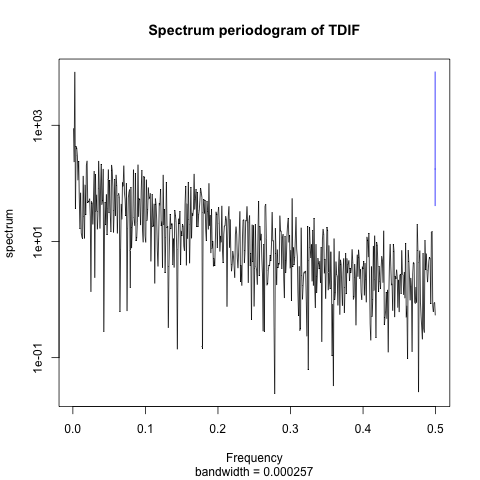
\includegraphics[width=6cm]{patt1.png}
\end{minipage}
\begin{minipage}[t]{0.48\textwidth}
\centering
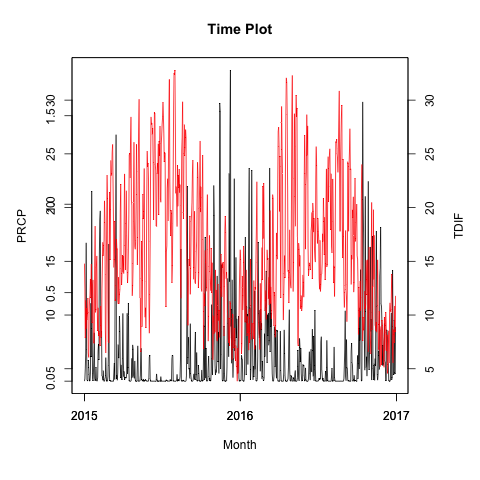
\includegraphics[width=6cm]{patt2.png}
\end{minipage}
\caption{Spectrum Plot and Time Plot}
\label{patt}
\end{figure}

On the right hand side is the time plot of TDIF (the red line) and PRCP (the black line). The red line shows a clear cycle per year, corresponding to the spectrum analysis before. On the other hand, no clear pattern of the black line can be observed. But it can tell us that PRCP is likely to be high when TDIF is low and vice versa. Overall even if we confirm the existence of a seasonal pattern in PRCP (which should be true), it may not play a crucial role in predicting daily weather. However, what we learn from the analysis above is, the TDIF is important in predicting PRCP and they are likely to be not positively, but negatively correlated.